\documentclass[12pt]{article}
\setlength{\textwidth}{17cm}
\setlength{\textheight}{24cm}
\setlength{\topmargin}{-2cm}
\setlength{\footskip}{1cm}
\setlength{\evensidemargin}{0cm}
\setlength{\oddsidemargin}{0cm}
\setlength{\parindent}{0cm}

\usepackage{allrunes}
\usepackage{amsmath}
\usepackage[english]{babel}
\usepackage[T1]{fontenc}
\usepackage[utf8]{inputenc}
\usepackage{fixltx2e}
\usepackage{multirow}

\usepackage[hyphens]{url}
\usepackage[unicode,colorlinks=true,breaklinks]{hyperref}
%\usepackage[dvips]{hyperref}
%should display links, but it does not work with \H accent
%and formulas in section titles

\hypersetup{colorlinks,linkcolor=blue,urlcolor=magenta,citecolor=magenta}
%Breaks long url`s in text, while keeping it one link:

\usepackage{amsfonts}
\usepackage{amsthm}
\usepackage{amssymb}


\theoremstyle{plain}
\usepackage{graphicx}

%\usepackage{gensymb}
\usepackage{float}

% For bra-ket notation
\usepackage{braket}

%% New commands
\newcommand{\dd}{\textrm{d}}

%% Pauli matrices
\newcommand{\sigx}{\sigma_x}
\newcommand{\sigy}{\sigma_y}
\newcommand{\sigz}{\sigma_z}

\newcommand{\paulix}{
    \left( \begin{array}{cc}
        0 & 1 \\
        1 & 0
    \end{array}
    \right)
}

\newcommand{\pauliy}{
    \left( \begin{array}{cc}
        0 & -i \\
        i & 0
    \end{array}
    \right)
}

\newcommand{\pauliz}{
    \left( \begin{array}{cc}
        1 & 0 \\
        0 & -1
    \end{array}
    \right)
}


\begin{document}
\title{16th exam item}
\author{András Mátyás Biricz}

\maketitle


\newpage
\begin{abstract}
    Többdimenziós adatok – Geográfiai és térbeli adatok reprezentálása, pontfelhők. Kere-sési alapproblémák: intervallum-keresés, térbeli keresés, legközelebbi szomszédok. Térbeli indexek, térkitöltő görbék (Z-index, Peano–Hilbert-index), kD-fa, R-fa, a bitkódolás sze-repe. Tércellázási módszerek: Delaunay-háromszögelés, Voronoi-cellázás. A gömb inde-xelése, Quad-tree, HEALPix, HTM.
    
    Multidimensional data - geographical and spatial data representation, point clouds. Basic searching algorithms: interval searching, spatial searching, nearest neighbours. Spatial indices, space filling curves (Z-index, Peano–Hilbert-index), kD-tree, R-tree, the role of binary coding. Spatial tesselation: Delaunay-triangulation, Voronoi-diagram. Pixelization of the sphere, quad-tree, HEALPix, HTM.
\end{abstract}


\section{Introduction}

As tehnology adavances it enables us to collect even more and more data about the world we live in. These datasets are diverse, can be simulational data or even results of measurements. For instance, these can be 3-dimensional with Euclidean metric or even higher dimensional such as phase space in time or other parameter spaces. The surface of the sphere is also a unique problem for us, since Earth is a round planet. :)

Some of the fundamental problems need to be adressed when dealing with these datasets are the following: 

\begin{itemize}
	\item finding points in a given region of space.
	\item Finding nearest neigbours of a point.
	\item Estimate the continuous density field from discrete points.
	\item Finding clusters.
	\item Interactive visualization of large point clouds.
\end{itemize}

\section{Spatial data representation}

Since storage systems are one dimensional, multi-dimensional data should be mapped to one dimension in order to represent them. This can be achieved by splitting a plane/space/hyperspace into cells somehow and by numbering these cells observing locality, which means close cells will have nearby numbers. For further processing, an index can be built on these cell numbers. 

A $k$-dimensional index can be a spatial index or even $k$ coordinates often with error. The simplest example is the case of Euclidean metric, where different scale can be set for each dimension.

\pagebreak

A $k$-dimensional indexing plan is as follows:

\begin{itemize}
	\item split space into small cells (grid, hierarchical tesselation, etc.).
	\item Number cells with integers (assign numbers observing data locality).
	\item For each data point, find corresponding cell.
	\item Tag data point with cell number.
	\item Build index on cell tags.
\end{itemize}

After this process points in a cell can be queried by scanning the index range, which is very fast.

In case of geographical data (Earth, sky) the representation can be given with spherical polar coordinates or 3D unit vectors or even some other methods described in the Geographic Information Systems (GIS). To read about the GIS please follow this link\footnote{\url{https://gisgeography.com/spatial-data-types-vector-raster/
}.}.

\section{Spatial indices}

Spatial indices are used by spatial databases to optimize spatial queries. These are the numbering methods of cells with integers in a special way to keep locality. The most common methods are the Z-index, Peano–Hilbert-index, k-d-tree, R-tree.

\subsection{Z-index}

The most widely used method is the Z-ordering, where the value of a point in a multi-dimensional space is simply calculated by interleaving the binary representations of its coordinate values (see figure \ref{zcurve}). Once the data are sorted into this ordering the points can be stored in a binary search tree and used directly, which is called a linear quadtree\footnote{\url{https://en.wikipedia.org/wiki/Z-order_curve}.}.

Quad-trees are most often used to partition a two-dimensional space by recursively subdividing it into four quadrants or regions. All forms of quadtrees share some common features:

\begin{itemize}
	\item they decompose space into adaptable cells.
	\item each cell has a maximum capacity, so when it is reached, the cell splits.
	\item The tree directory follows the spatial decomposition of the quadtree.
\end{itemize}

The resulting tree is not balanced, that means empty leaf cells can be found (see figure \ref{quadtree}). The 3-dimensional version of the quadtree is the octree (see figure \ref{octree}). 

\pagebreak

\begin{figure}[h!]
    \centering
	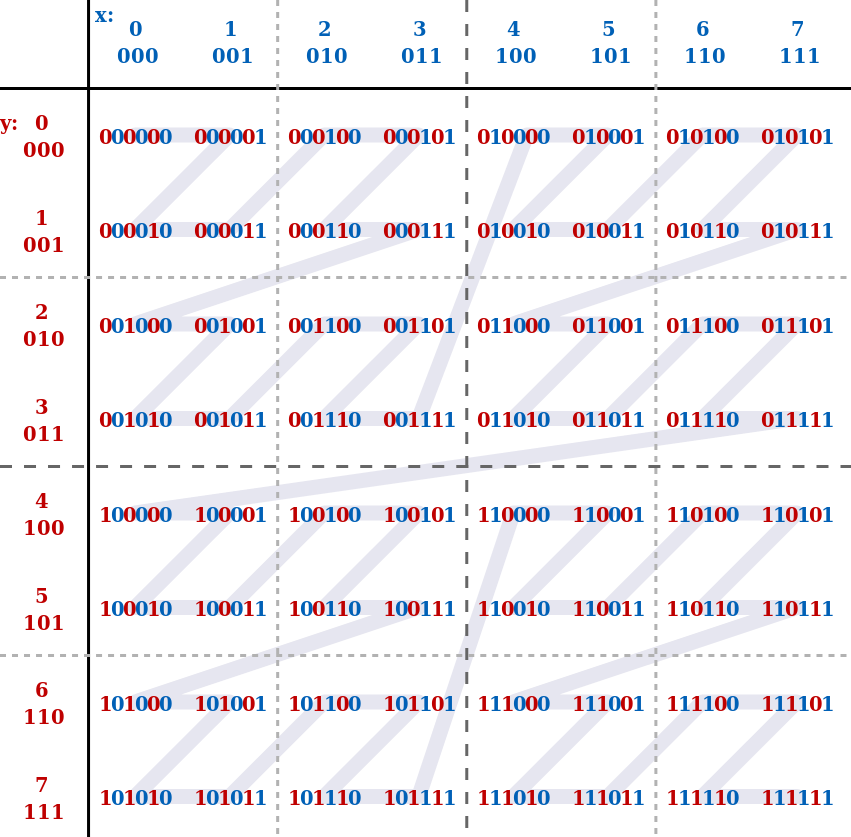
\includegraphics[width=.9\linewidth]{media/Z-curve.png}
	\caption{Illustration of the Z-values for the two dimensional case with integer coordinates $0 \leq x \leq 7$, $0 \leq y \leq 7$. The source was accessed in June 2019 (\url{https://en.wikipedia.org/wiki/File:Z-curve.svg}).}
	\label{zcurve}
\end{figure}
\newpage

\begin{figure}[h!]
    \centering
	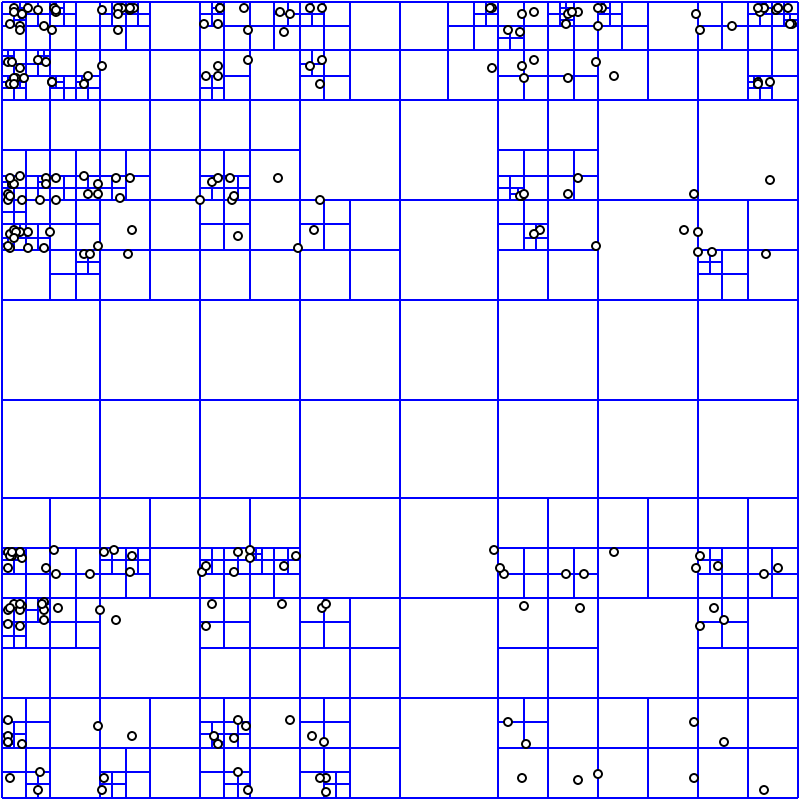
\includegraphics[width=.625\linewidth]{media/800px-Point_quadtree.png}
	\caption{A point-region quadtree with point data and a bucket capacity 1. The source was accessed in June 2019 (\url{https://en.wikipedia.org/wiki/Quadtree\#/media/File:Point_quadtree.svg}).}
	\label{quadtree}
\end{figure}

\begin{figure}[h!]
    \centering
	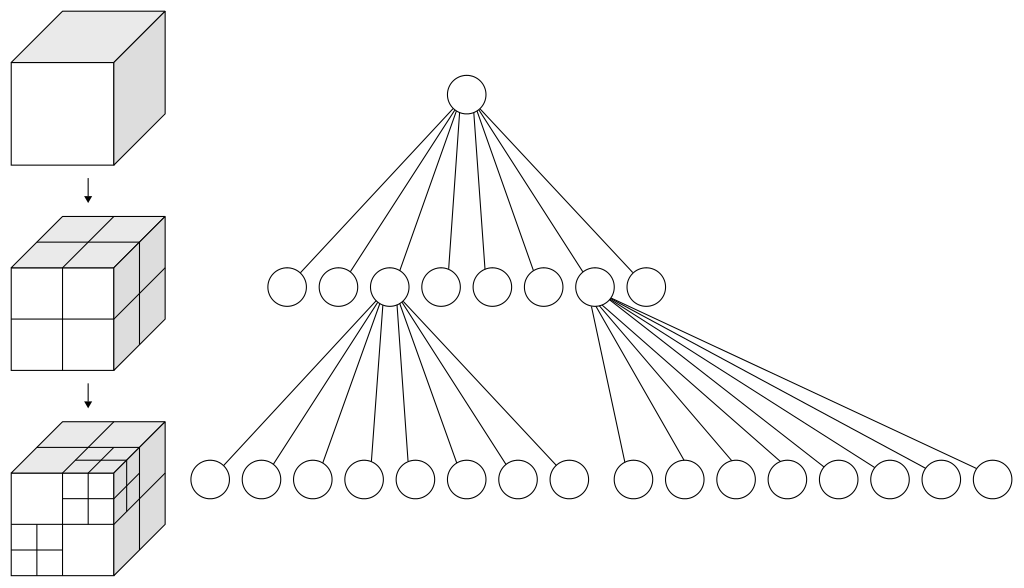
\includegraphics[width=.625\linewidth]{media/Octree2.png}
	\caption{Recursive subdivision of a cube into octants. The source was accessed in June 2019 (\url{https://en.wikipedia.org/wiki/Octree\#/media/File:Octree2.svg}).}
	\label{octree}
\end{figure}

\newpage

\subsection{Peano-Hilbert-index}

The Peano-Hilbert curve can be used to index the 2D or 3D space (see figure \ref{PHcurve}), because it has a space-filling behaviour, its length grows exponentially with iterations, has better locality than Z-ordering and its binary representation also reflects hierarchy. Note, that it is not a fractal. 

\begin{figure}[h!]
   \centering
	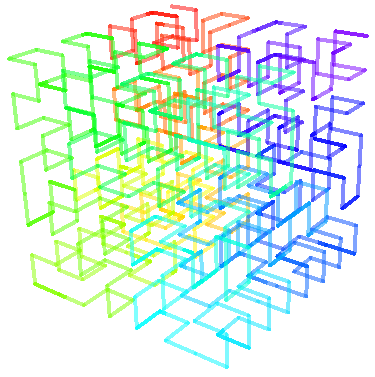
\includegraphics[width=.6\linewidth]{media/Hilbert3d-step3.png}
	\caption{Illustration of the Peano-Hilbert curve filing the 3-dimensional space. The source was accessed in June 2019 (\url{https://en.wikipedia.org/wiki/File:Hilbert3d-step3.png}).}
	\label{PHcurve}
\end{figure}

\subsection{k-d-tree}

A k-d tree (short for k-dimensional tree) is a space-partitioning data structure for organizing points in a k-dimensional space (see figure \ref{kdtree_1}). k-d trees are a useful data structure for several applications, such as searches involving a multidimensional search key (e.g. range searches and nearest neighbor searches). k-d trees are a special case of binary space partitioning trees\footnote{\url{https://en.wikipedia.org/wiki/K-d_tree}.}.

The algorithm to build a k-d tree is as follows:

\begin{itemize}
	\item find bounding box.
	\item Find median along first dimension.
	\item Split box into half at median.
	\item Repeat recursively for both new boxes.
\end{itemize}

Since median requires sort it is an expensive step and therefore usually estimated with average. This tree method is efficient in higher dimensions. The cell ID binary representation follows tree hierarcy (see figure \ref{kdtree_2}). 


\begin{figure}[h!]
    \centering
	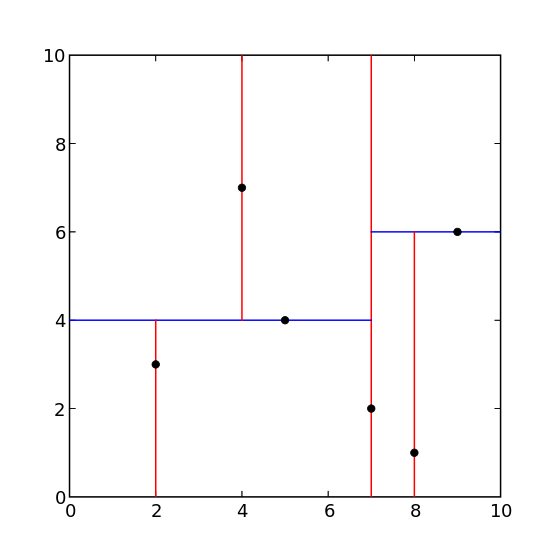
\includegraphics[width=.6\linewidth]{media/Kdtree_2d.png}
	\caption{k-d tree decomposition for the point set (2,3), (5,4), (9,6), (4,7), (8,1), (7,2). The source was accessed in June 2019 (\url{https://en.wikipedia.org/wiki/File:Tree_0001.svg}).}
	\label{kdtree_1}
\end{figure}

\begin{figure}[h!]
    \centering
	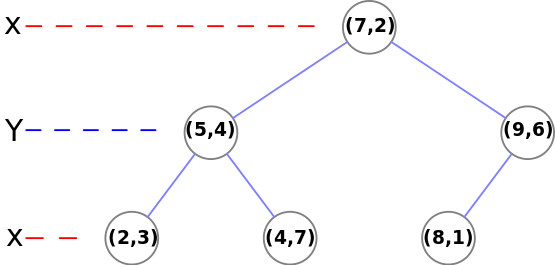
\includegraphics[width=.6\linewidth]{media/Tree_0001.png}
	\caption{The resulting k-d tree. The source was accessed in June 2019 (\url{https://en.wikipedia.org/wiki/File:Kdtree_2d.svg}).}
	\label{kdtree_2}
\end{figure}


\pagebreak
\subsection{R-tree}

R-trees are tree data structures used for indexing multi-dimensional data such as geographical coordinates, rectangles or polygons. The R-tree was proposed by \hyperlink{R. Guttmann (1984)}{R. Guttmann (1984)} and became significant in both theoretical and applied contexts. A common real-world usage for an R-tree might be to store spatial objects such as restaurant locations or the polygons that typical maps are made of: streets, buildings, outlines of lakes, coastlines, etc. and then find answers quickly to queries such as "Find all museums within 2 km of my current location" or "retrieve all road segments within 2 km of my location".

The key idea of the data structure is to group nearby objects and represent them with their minimum bounding rectangle in the next higher level of the tree (see figure \ref{rtree}); the "R" in R-tree is for rectangle. Since all objects lie within this bounding rectangle, a query that does not intersect the bounding rectangle also cannot intersect any of the contained objects. At the leaf level, each rectangle describes a single object; at higher levels the aggregation of an increasing number of objects. This can also be seen as an increasingly coarse approximation of the data set.

\begin{figure}[h!]
    \centering
	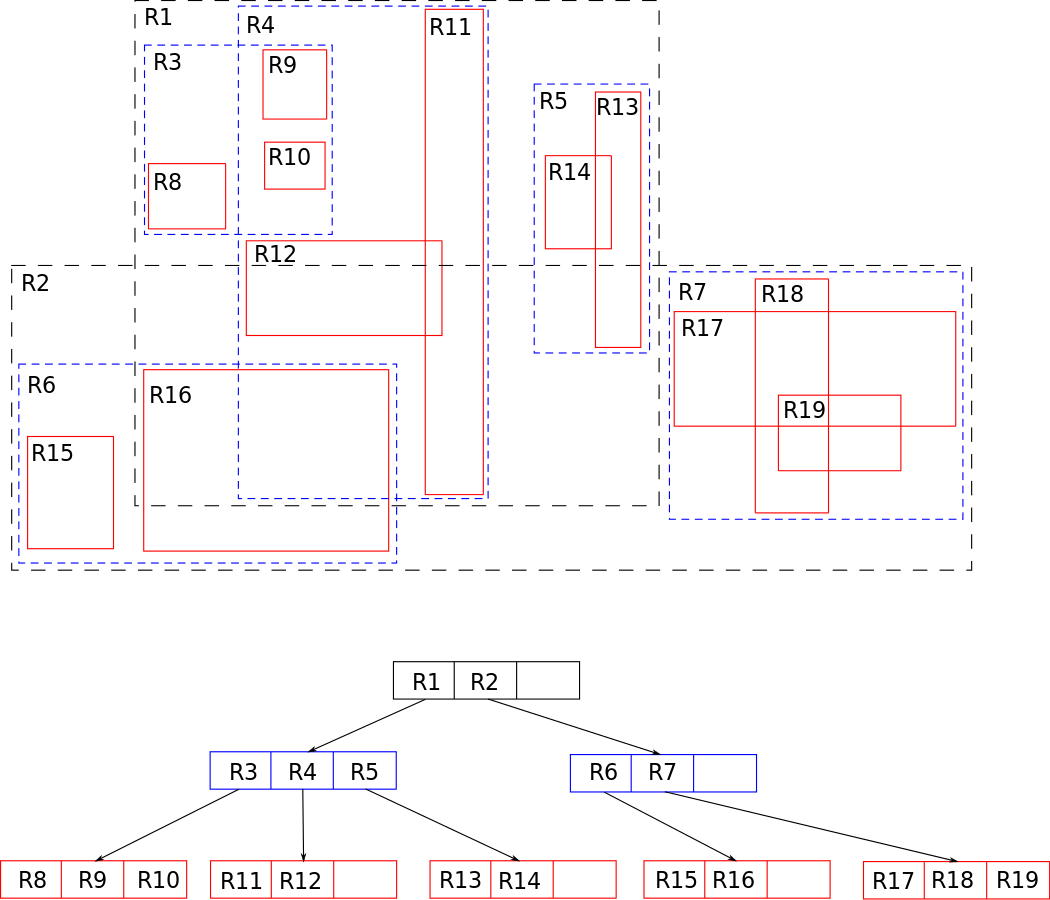
\includegraphics[width=.6\linewidth]{media/R-tree.png}
	\caption{Simple example of an R-tree for 2D rectangles. The source was accessed in June 2019 (\url{https://en.wikipedia.org/wiki/File:Kdtree_2d.svg}).}
	\label{rtree}
\end{figure}

%

The source and further information can be found here\footnote{\url{https://en.wikipedia.org/wiki/R-tree}.}

%https://en.wikipedia.org/wiki/Spatial_database

%
%https://www.forceflow.be/2013/10/07/morton-encodingdecoding-through-bit-interleaving-implementations/

%

%

%

%https://en.wikipedia.org/wiki/Space-filling_curve

%http://wwwmayr.informatik.tu-muenchen.de/konferenzen/Jass05/courses/2/Valgaerts/Valgaerts_paper.pdf

%https://www.forceflow.be/2013/10/07/morton-encodingdecoding-through-bit-interleaving-implementations/

%https://en.wikipedia.org/wiki/Binary_code

\pagebreak
\section{Space tesselation}

The space tesselation is the process how the multi-dimensional space or the surface of the sphere is split into cells. There exist single-level or multi-level tesselations, hierarchical or even adaptive tesselations. In case of grid, the cells are usually defined by orthogonal vectors, where different scales are possible along different axes. It has advantages that its structure is well defined and the cell vertices are easy to compute, but on the other hand the number of cells is very high in higher dimensions and it is non-adaptive, that means there can be a lots of almost empty and crowded cells. There exist better methods for tesselation, for example the Delaunay-triangulation or the Voronoi diagram.

\subsection{Delaunay, Voronoi}

A very popular computational geometry problem is the Voronoi Diagram (VD), and its dual Delaunay Triangulation (DT). In both cases, the input is a set of points (sites) (see figure \ref{delavoro}). In VD, the output is a tessellation of the space into convex polygons, as one per input site, such that each polygon covers all locations that are closest to the corresponding site than any other site. In DT, the output is a triangulation, where each triangle connects three sites, such that the circumcircle of each triangle does not contain any other sites. These two constructs are dual in a sense that each edge in the DT connects two sites that share a common edge in VD.

The source and more information can be found here \footnote{\url{http://aseldawy.blogspot.com/2015/12/voronoi-diagram-and-dealunay.html}.}.

\begin{figure}[h!]
    \centering
	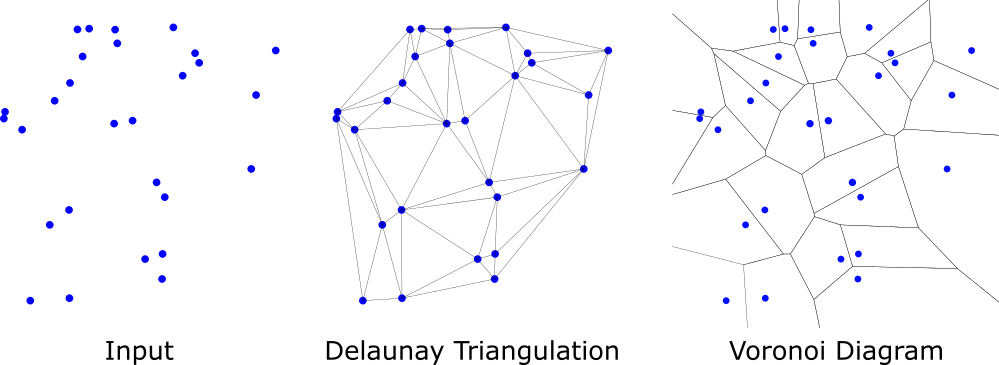
\includegraphics[width=.9\linewidth]{media/delavoro.png}
	\caption{Illustration of the Delaunay-triangulation and the Voronoi-diagram. The source was accessed in June 2019 (\url{http://aseldawy.blogspot.com/2015/12/voronoi-diagram-and-dealunay.html}).}
	\label{delavoro}
\end{figure}



%https://www.geos.ed.ac.uk/~gisteac/gis_book_abridged/files/ch36.pdf

%https://en.wikipedia.org/wiki/Delaunay_triangulation

%https://en.wikipedia.org/wiki/Voronoi_diagram


\subsection{Pixelization of the sphere}

The topology of the surface of the sphere eventuates that the indexing is far from being trivial. The simple, usual indexing suffers from numerical instability around the poles due to singularities and also from discontinuity at $- 180^\circ - + 180^\circ$. These problems should be addressed algorithmically. The most frequent solution is to use Cartesian unit vectors instead of spherical coordinates, but a more advanced approach can be used: tessellate surface, tag cells with numbers and assign data points to cells, index them by the cell IDs. Earlier methods can be generalized (Quad-tree, Voronoi), but due to the periodic topology the algorithms should be modified. The two most used methods are the Hierarchical Triangular Mesh (HTM) and Hierarchical Equal Area isoLatitude Pixelisation (HEALPix) approaches. 

\subsubsection{HTM}

The Hierarchical Triangular Mesh is a multi-level, recursive decomposition of the sphere (\hyperlink{Gorski et al. (2005)}{Gorski et al. (2005)}). It starts with an octahedron and we call “level 0 trixels“ each of its eight equilateral triangle faces. Each trixel can then be split into four smaller trixels by introducing new vertices at the midpoints of each side. Trixel division repeats recursively and indefinitely to produce smaller and smaller trixel\footnote{\url{https://kronuz.io/Xapiand/docs/reference-guide/schemas/field-types/geospatial-type/htm/}.}. The result is a Quad-tree on the sphere (see figure \ref{htm}).

\begin{figure}[h!]
    \centering
	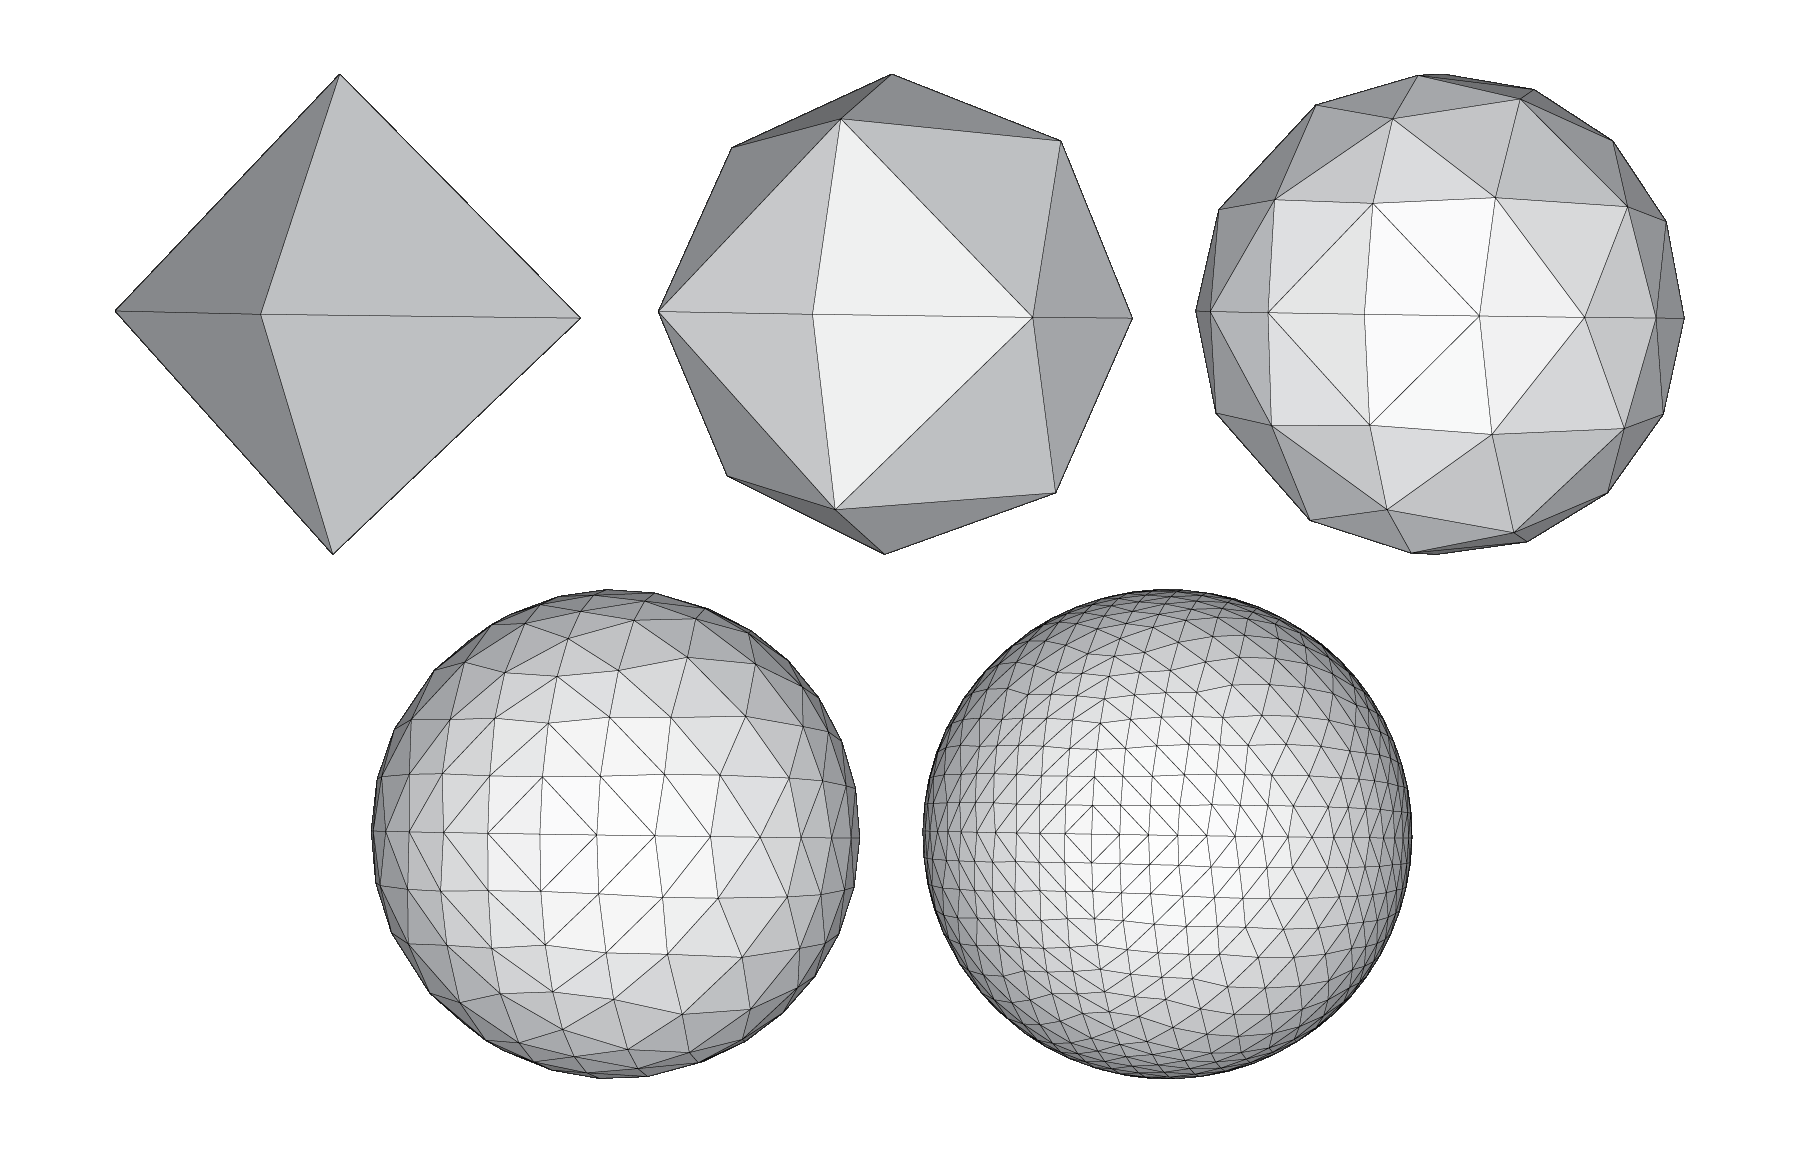
\includegraphics[width=.9\linewidth]{media/htm.png}
	\caption{Illustration of the Hierarchical Triangular Mesh at different iterations. The source was accessed in June 2019 (\url{https://kronuz.io/Xapiand/docs/reference-guide/schemas/field-types/geospatial-type/htm/}).}
	\label{htm}
\end{figure}

The advantage of this method is that it is easy to compute and it allows quick search, but on the other hand the region search algorithms are quite complex and the triangle size and shape varies slightly around the sphere.

\pagebreak
\subsubsection{HEALPix}

The Hierarchical Equal Area isoLatitude Pixelization (HEALPix) scheme of the sphere produces a subdivision of a spherical surface in which each pixel covers the same surface area as every other pixel (\hyperlink{Gorski et al. (2005)}{Gorski et al. (2005)}). Few iterations can be seen on figure \ref{HEALPix_spheres}.

\begin{figure}[h!]
    \centering
	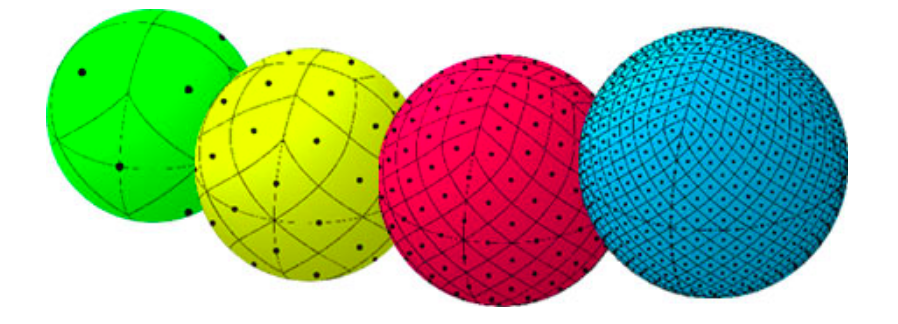
\includegraphics[width=.65\linewidth]{media/HEALPix_spheres.png}
	\caption{The green sphere represents the lowest resolution possible with the HEALPix base partitioning of the sphere surface into 12 equal sized pixels. The yellow sphere has a HEALPix grid of 48 pixels, the red sphere has 192 pixels, and the blue sphere has a grid of 768 pixels (7.3 degree resolution). Source: \url{https://healpix.jpl.nasa.gov/}.}
	\label{HEALPix_spheres}
\end{figure}

%https://rts2.org/malaga/pres/L_Nicastro.pdf




\section{Searching Algorithms}

Searching Algorithms are designed to check for an element or retrieve an element from any data structure where it is stored. Based on the type of search operation, these algorithms are generally classified into two categories\footnote{\url{https://www.geeksforgeeks.org/searching-algorithms/}.}:

\begin{itemize}
	\item \textbf{Sequential search:} the list or array is traversed sequentially and every element is checked. For example: linear search.
	\item \textbf{Interval search:} These algorithms are specifically designed for searching in sorted data-structures. These type of searching algorithms are much more efficient than linear search as they repeatedly target the center of the search structure and divide the search space in half. For example: binary search.
\end{itemize}


%https://www.geeksforgeeks.org/searching-algorithms/

\subsection{Spatial search}

The spatial search takes advantage of the properties of the spatial databases and use spatial indices to find the target. The search region is given with analytic description and during the searching process the cells are compared with the search region with the following possible outcomes:

\begin{itemize}
	\item cell is entirely inside $\rightarrow$ all points are matches,
	\item Cell is entirely outside $\rightarrow$ no points are matches.
	\item Cell intersects with region $\rightarrow$ have to test each point.
\end{itemize}

The spatial search is efficient if the number of cells is much less than the number of data points. Roughly, the number of cells should be around $\sqrt[3]{N}$, where $N$ is the number of points in total.

\subsection{K-nearest neighbour search}

In order to find the K-nearest neighbours of a query point in a d-dimensional space spatial indices can be used. It is advantageous, because there is no need to compute distances from all data points, but on the other hand the closest point can be in the same cell as the query point or in the neighbouring cells. In high dimension, almost all cells are neighbours, so practically cells are to be used if the number of points is high ($N > 2^d$). The algorithm is as follows:

\begin{itemize}
	\item given a query point $Q$.
	\item Find cell $C$ for which $Q \in C$.
	\item Compute distance of all points $P \in C$. 
	\item Sort by distance, find $k^{\text{th}}$ closest.
	\item If the $k^{\text{th}}$ closest is further than any side of $C$ from $Q$, use neighbouring cells, too. 
	\item Also use neighbouring cells if there are less points in $C$ than $k$.
\end{itemize}

%https://en.wikipedia.org/wiki/Nearest_neighbor_search

\section{Conclusion}

In this exam item we learnt about the spatial databases, spatial tesselation, spatial indices and searching methods that take advantage of the properties of these special databases.

\newpage

\begin{thebibliography}{Nature}
%\bibliography{references}

\bibitem{Dobos_database_en}\hypertarget{Dobos_database_en}{}Dobos L. Design and implementation of scientific databases. Eötvös Loránd University, Dept. of Physics of Complex Systems, 2015. \url{http://www.vo.elte.hu/~dobos/teaching/scidb2016/scidb_en.pdf}

\bibitem{R. Guttmann (1984)}\hypertarget{R. Guttmann (1984)}{}
R. Guttmann. A dynamic index structure for spatial searching. In \textit{Proc. ACM SIGMOD}, pages 47-57, 1984.

\bibitem{A. S. Szalay et al (2007)}\hypertarget{A. S. Szalay et al (2007)}{}
A. S. Szalay, J. Gray, G. Fekete, P. Z. Kunszt, P. Kukol, and A. Thakar. Indexing the Sphere with the Hierarchical Triangular Mesh. \textit{Computing Research Repository}, pages 58–65, 2007.

\bibitem{Gorski et al. (2005)}\hypertarget{Gorski et al. (2005)}
Gorski, K.M., Hivon, E., Banday, A.J., Wandelt, B.D., Hansen, F.K., et al., HEALPix - a framework for high resolution discretization, and fast analysis of data distributed on the sphere. \textit{The Astrophysical Journal} \textbf{622}, 759–771. 2005.

\end{thebibliography}

\end{document}
